% Foliensatz: "AFu-Kurs nach DJ4UF" von DK0TU, Amateurfunkgruppe der TU Berlin
% Lizenz: CC BY-NC-SA 3.0 de (http://creativecommons.org/licenses/by-nc-sa/3.0/de/)
% Autoren:
% Lars Weiler <dc4lw@darc.de>

\documentclass[aspectratio=169]{beamer}

\usepackage[ngerman]{babel} % deutsche Worttrennung etc.
\usepackage[utf8]{inputenc} % UTF8 Text

\usepackage[super, comma, numbers, square, sort]{natbib}

\usepackage{hyperref}       % Hyperref Package für bessere Referenzen (todo)
\hypersetup{
	colorlinks=false,       %   false: boxed links; true: colored links
    %linkcolor=white,       %   color of internal links (change box color with linkbordercolor)
    citecolor=red,          %   color of links to bibliography
    filecolor=white,        %   color of file links
    urlcolor=blue           %   color of external links
}

\usepackage{multirow}
\usepackage{wasysym}  % Math Symbols like \permil
%\usepackage{colortbl}
%\usepackage{subscript}
%\usepackage{caption}
%\usepackage{setspace}
%\usepackage{xcolor}        % benutze CodeListe

% Footnote
%\usepackage{hanging}
%
%\setbeamertemplate{footnote}{%
%  \hangpara{2em}{1}%
%  \makebox[2em][l]{\insertfootnotemark}\footnotesize\insertfootnotetext\par%
%}


%\usepackage{pgf}
%\usepackage{tikz}
%\usetikzlibrary{arrows,automata}
%\usetikzlibrary{positioning}
%
%\tikzset{
%    state/.style={
%           rectangle,
%           rounded corners,
%           draw=black, very thick,
%           minimum height=2em,
%           minimum width=2pt,
%           inner sep=2pt,
%           text centered,
%           },
%}

%\usepackage{listings}
%\lstset{basicstyle=\small, numberstyle=\tiny, extendedchars=true, numbers=left, numbersep=5pt}
%\lstset{showtabs=false, showspaces=false, showstringspaces=false}
%%\lstset{backgroundcolor=\color{white!75!lightgray}, , frame=single}
%%\lstset{backgroundcolor=\color{white}}
%%\lstset{backgroundcolor=none}
%\lstset{keywordstyle=\color{blue!50!gray},  identifierstyle=\color{black}}
%\lstset{commentstyle=\color{green!50!gray}, stringstyle=\color{red!50!gray}}
%\lstset{language=C, fontadjust=true, tabsize=2, breaklines=true}
%\lstset{backgroundcolor=\color{white!75!lightgray}, caption=\lstname, frame=single}
%\lstset{emphstyle=\color{black}\fbox}
%
%% Keine "Listing:"-Caption
%\captionsetup{labelformat=empty,labelsep=none}
%
%% für mathematische Umgebungen
%\usepackage{amsmath,amsfonts,amssymb}
%
%\lstdefinestyle{Bash}{
%language=Bash,
%frame=single,
%rulecolor=\color{black},
%backgroundcolor=\color{gray!50},
%keywordstyle=\color{black},
%identifierstyle=,
%commentstyle=\color{black},
%stringstyle=\color{magenta!65!white},
%showstringspaces=false,
%basicstyle=\footnotesize\ttfamily\color{black},
%numbers=none,
%breaklines=true,
%captionpos=b
%}

%\usepackage{listings}
%
%\lstdefinestyle{basic}{
%    captionpos=t,%
%    basicstyle=\footnotesize\ttfamily,%
%    numberstyle=\tiny,%
%    numbers=left,%
%    stepnumber=1,%
%    frame=single,%
%    showspaces=false,%
%    showstringspaces=false,%
%    showtabs=false,%
%    %
%    keywordstyle=\color{blue},%
%    identifierstyle=,%
%    commentstyle=\color{gray},%
%    stringstyle=\color{magenta}%
%}



% fließende Boxen haben keinen Abstand
%\fboxsep0mm

% inkludiere Creative Commons Helper
%%%%%%%%%%%%%%%%%%%%%%%%%%%%%%%%%%%%%%%%%%%%%%%%%%%%%%%%%%%%%%%%
%% ccBeamer 0.1, 2007-07-02                                   %%
%% Written by Sebastian Pipping <webmaster@hartwork.org>      %%
%% ---------------------------------------------------------- %%
%% Licensed under Creative Commons Attribution-ShareAlike 3.0 %%
%% http://creativecommons.org/licenses/by-sa/3.0/             %%
%%%%%%%%%%%%%%%%%%%%%%%%%%%%%%%%%%%%%%%%%%%%%%%%%%%%%%%%%%%%%%%%


%% Images
\newcommand{\CcImageBy}[1]{%
	
\includegraphics[scale=#1]{texdata/creative_commons/cc_by_30.pdf}%
}
\newcommand{\CcImageCc}[1]{%
	
\includegraphics[scale=#1]{texdata/creative_commons/cc_cc_30.pdf}%
}
\newcommand{\CcImageDevNations}[1]{%
	
\includegraphics[scale=#1]{texdata/creative_commons/cc_dev_nations_30.pdf}%
}
\newcommand{\CcImageNc}[1]{%
	
\includegraphics[scale=#1]{texdata/creative_commons/cc_nc_30.pdf}%
}
\newcommand{\CcImageNd}[1]{%
	
\includegraphics[scale=#1]{texdata/creative_commons/cc_nd_30.pdf}%
}
\newcommand{\CcImagePd}[1]{%
	
\includegraphics[scale=#1]{texdata/creative_commons/cc_pd_30.pdf}%
}
\newcommand{\CcImageSa}[1]{%
	
\includegraphics[scale=#1]{texdata/creative_commons/cc_sa_30.pdf}%
}
\newcommand{\CcImageSampling}[1]{%
	
\includegraphics[scale=#1]{texdata/creative_commons/cc_sampling_30.pdf}%
}
\newcommand{\CcImageSamplingPlus}[1]{%
	
\includegraphics[scale=#1]{texdata/creative_commons/cc_sampling_plus_30.pdf}%
}


%% Groups
\newcommand{\CcGroupBy}[2]{% zoom, gap
	\CcImageCc{#1}\hspace*{#2}\CcImageBy{#1}%
}
\newcommand{\CcGroupByNc}[2]{% zoom, gap
	\CcImageCc{#1}\hspace*{#2}\CcImageBy{#1}\hspace*{#2}\CcImageNc{#1}%
}
\newcommand{\CcGroupByNcNd}[2]{% zoom, gap
	\CcImageCc{#1}\hspace*{#2}\CcImageBy{#1}\hspace*{#2}\CcImageNc{#1}\hspace*{#2}\CcImageNd{#1}%
}
\newcommand{\CcGroupByNcSa}[2]{% zoom, gap
	\CcImageCc{#1}\hspace*{#2}\CcImageBy{#1}\hspace*{#2}\CcImageNc{#1}\hspace*{#2}\CcImageSa{#1}%
}
\newcommand{\CcGroupByNd}[2]{% zoom, gap
	\CcImageCc{#1}\hspace*{#2}\CcImageBy{#1}\hspace*{#2}\CcImageNd{#1}%
}
\newcommand{\CcGroupBySa}[2]{% zoom, gap
	\CcImageCc{#1}\hspace*{#2}\CcImageBy{#1}\hspace*{#2}\CcImageSa{#1}%
}
\newcommand{\CcGroupDevNations}[2]{% zoom, gap
	\CcImageCc{#1}\hspace*{#2}\CcImageDevNations{#1}%
}
\newcommand{\CcGroupNcSampling}[2]{% zoom, gap
	\CcImageCc{#1}\hspace*{#2}\CcImageNc{#1}\hspace*{#2}\CcImageSampling{#1}%
}
\newcommand{\CcGroupPd}[1]{% zoom
	\CcImagePd{#1}%
}
\newcommand{\CcGroupSampling}[1]{% zoom
	\CcImageSampling{#1}%
}
\newcommand{\CcGroupSamplingPlus}[1]{% zoom
	\CcImageSamplingPlus{#1}%
}


%% Text
\newcommand{\CcLongnameBy}{Attribution}
\newcommand{\CcLongnameByNc}{Attribution-NonCommercial}
\newcommand{\CcLongnameByNcNd}{Attribution-NoDerivs}
\newcommand{\CcLongnameByNcSa}{Attribution-NonCommercial-ShareAlike}
\newcommand{\CcLongnameByNd}{Attribution-NoDerivs}
\newcommand{\CcLongnameBySa}{Attribution-ShareAlike}

\newcommand{\CcNote}[1]{% longname
	This work is licensed under the \textit{Creative Commons #1 3.0 License}.%
}


% generelles Thema auswählen
\usetheme{Goettingen} %Berlin spart ohne Sidebar allerdings angenehm Platz
% AnnArbor | Antibes | Bergen | Berkeley | Berlin | Boadilla | boxes | CambridgeUS | Copenhagen | Darmstadt | default | Dresden | Frankfurt | Goettingen | Hannover | Ilmenau | JuanLesPins | Luebeck | Madrid | Malmoe | Marburg | Montpellier | PaloAlto | Pittsburgh | Rochester | Singapore | Szeged | Warsaw

% Farben wählen
\usecolortheme{beetle}
% beaver | beetle | crane | default | dolphin | dove | fly | lily | orchid | rose | seagull | seahorse | sidebartab | structure | whale | wolverine

% Setze alle Farben auf Grau und Weiß
%\definecolor{craneorange}{RGB}{64,64,64}
%\definecolor{craneblue}{RGB}{255,255,255}

% Schriftart wählen
\usefonttheme{default}
% default | professionalfonts | serif | structurebold | structureitalicserif | structuresmallcapsserif

% Innere Themen(Kopf-, Fuß-, Sidebar usw)
%\useinnertheme{default}
\useinnertheme{circles}
% default | inmargin | rectangles | rounded | circles

% Äußere Themen (Anordnung der inneren, grenzen der Folien etc.)
\useoutertheme{infolines}
% default | infolines | miniframes | shadow | sidebar | smoothbars | smoothtree | split | tree

% Deaktiviere Navigations-Symbole ({} -> leer)
\setbeamertemplate{navigation symbols}{}
%\setbeamertemplate{navigation symbols}{\large \ifnum \insertframenumber <10 0\fi\insertframenumber/\inserttotalframenumber\vspace*{0.2ex}}

% Zeige ein Hintergrundbild
\setbeamertemplate{background canvas}{
        \hspace*{-2.0cm}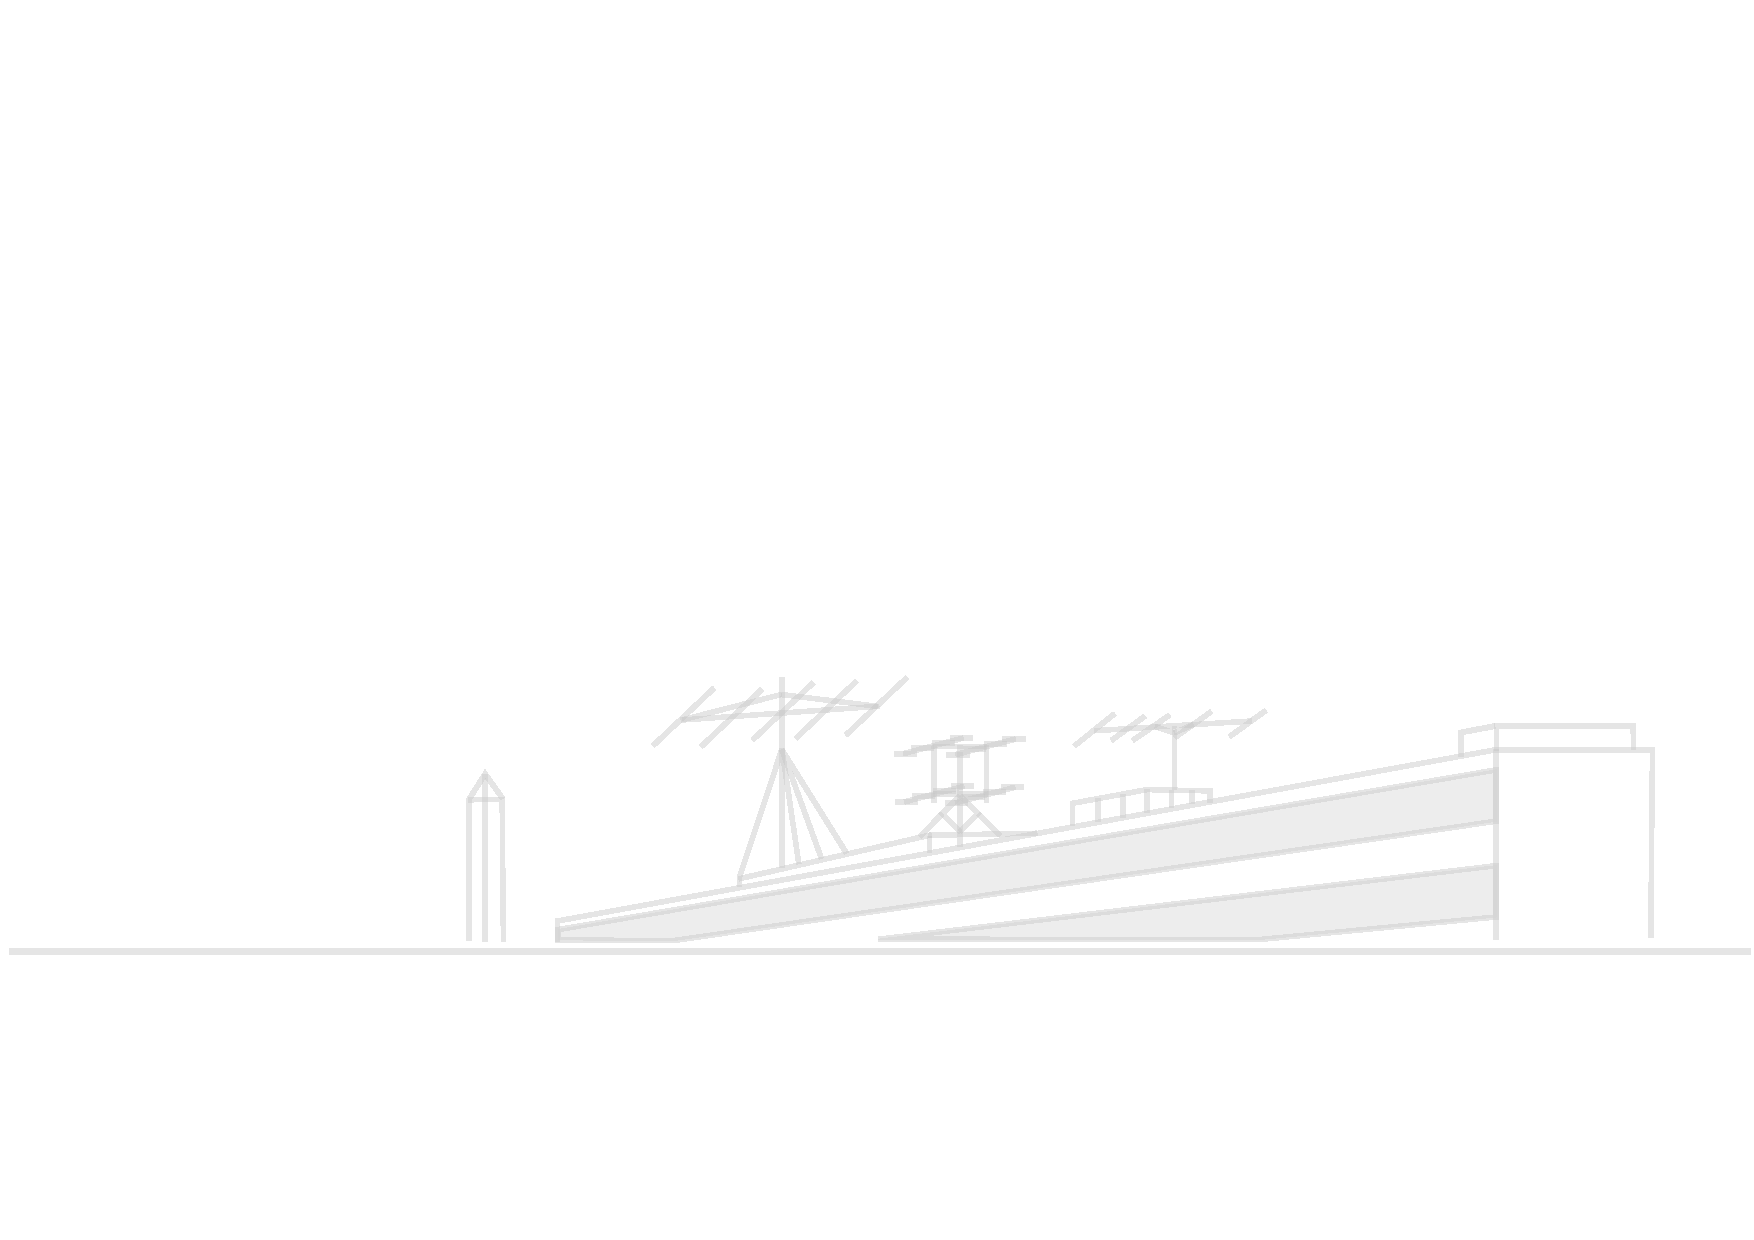
\includegraphics[width=17.8cm]{texdata/dk0tu_rooftop_background.pdf}
}

% Foliennummer einfügen
\setbeamertemplate{footline}[frame number]
%\setbeamertemplate{footline}{}

% Ändere das Zeichen vor jedem item
%\setbeamertemplate{itemize item}{\color{craneorange}$\blacktriangleright$}
%\setbeamertemplate{itemize subitem}{\color{craneorange}$\triangleright$}
%\setbeamertemplate{itemize subsubitem}{\color{craneorange}$\blacktriangleright$}

% Ändert die Blöcke 
\setbeamertemplate{blocks}[rounded][shadow=true]
% default | rounded [shadow=true|false]

%
% Eigene Kommandos
%

% Hack to get natbib and beamer working together. "The beamer user guide suggests
% that only the manual bibliography entry approach is supported"
% on some system it works out of the box, sometimes you need the hack :-(
% so check it --dl7bst
\ifdefined\newblock
    \relax
\else
    \newcommand{\newblock}{}
\fi

% \includedia command to generate png out of a dia file
% NEEDS installed dia and pdflatex option --shell-escape
\newcommand{\includedia}[1]{
    \immediate\write18{/usr/bin/dia #1.dia -e #1_diatmp.png -t png}
}

% RICHIG GROSSER FONT!
\newfont{\bigfont}{cmr10 at 144pt}
\newfont{\smallfont}{cmr10 at 8pt}

% Römische Ziffern
\makeatletter
\newcommand{\rmnum}[1]{\romannumeral #1}
\newcommand{\Rmnum}[1]{\expandafter\@slowromancap\romannumeral #1@}
\makeatother

% Schwarze Überschrift
%\setbeamercolor{frametitle}{fg=black}
%\setbeamercolor{title}{fg=black}

% Item- und Box-Farben
\definecolor{deepBlue}{HTML}{000066}
\setbeamercolor{itemize item}{fg=deepBlue}
\setbeamercolor{itemize subitem}{fg=deepBlue}
\setbeamercolor{description item}{fg=deepBlue}
\setbeamercolor{block title}{fg=deepBlue!100, bg=blue!15}
\setbeamercolor{block body}{fg=black, bg=blue!5}
\setbeamercolor{block title alerted}{fg=deepBlue, bg=red!75}
\setbeamercolor{block body alerted}{fg=black, bg=red!15}
\setbeamercolor*{block title example}{fg=blue!50, bg=blue!10}
\setbeamercolor*{block body example}{fg= blue, bg=blue!5}

%\setbeamercolor{section in head/foot}{parent=palette primary}
%\setbeamercolor{subsection in head/foot}{parent=palette secondary}
%\setbeamercolor{sidebar}{fg=darkblue,bg=yellow!90!orange}
%\setbeamercolor{title in sidebar}{fg=darkblue}
%\setbeamercolor{author in sidebar}{fg=darkblue}
%\setbeamercolor{section in sidebar}{fg=darkblue!10!black}
%\setbeamercolor{subsection in sidebar}{fg=darkblue!50!black}

% Titlepage Infos
\title{AFu-Kurs nach DJ4UF}
\author[DKØTU]{DKØTU\\ \footnotesize{Amateurfunkgruppe der TU Berlin}}
\institute[DKØTU]{\url{http://www.dk0tu.de} }

% PDF-Eigenschaften
\subject{DK0TU-Amateurfunkkurs nach DJ4UF}
\keywords{Amateurfunk Kurs HAM Radio Course CC-BY-NC-SA OpenSource TU Berlin DK0TU}

\subtitle{Technik A15: \\
           Übertragungstechnik \\[2em]}
\date{Stand 07.03.2016}
 \begin{document}

\begin{frame}
    \titlepage
    \vfill
    \begin{center}
        \ccbyncsaeu\\
        {\tiny This work is licensed under the \em{Creative Commons Attribution-NonCommercial-ShareAlike 3.0 License}.}\\[0.5ex]
         \tiny Amateurfunkgruppe der Technische Universität Berlin (AfuTUB), DKØTU
         %\includegraphics[scale=0.5]{img/DK0TU_Logo.pdf}
    \end{center}
\end{frame}


\begin{frame}{Einleitung / Umleitung}
  Aufgrund sehr großer Überschneidungen werden viele Digimodes bereits in der \emph{Lektion E16: (Digitale) Betriebsarten} behandelt.
\end{frame}

\section{Digitalsignal}
\begin{frame}{Analog-Digital-Wandlung (ADC)}
  \begin{columns}
    \column{.5\textwidth}
    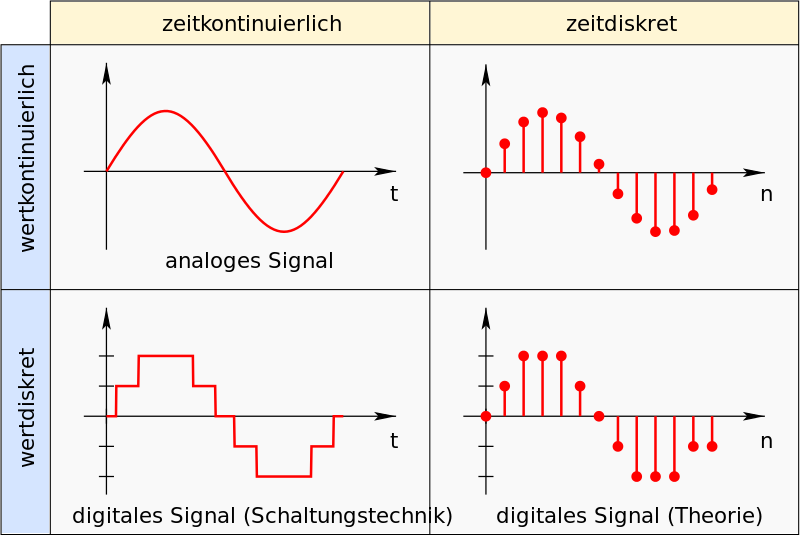
\includegraphics[width=\textwidth,height=.8\textheight,keepaspectratio]{a15/Uebersicht_kontinuierliche_und_diskrete_Signale.png}\\
    {\tiny Kontinuierliche und diskrete Signale \hyperlink{refs}{\cite{wm}}}
    \column{.45\textwidth}
    Ein analoges Signal wird in ein digitales Signal über zwei Schritte umgewandelt
    \begin{description}
      \item[Abtastung] zeitkontinuierlich $\rightarrow$ zeitdiskret
      \item[Quantisierung] wertkontinuierlich $\rightarrow$ wertdiskret
    \end{description}
    \begin{block}{Nyquist-Shannon-Abtasttheorem}
      $T_A \leq \cfrac{1}{2 \cdot f_{max}}$\\[.5em]
      $T_A$: Abtastfrequenz\\
      $f_{max}$: Maximale Informationsfrequenz
    \end{block}
  \end{columns}
\end{frame}

\begin{frame}{Kodierung}
  Je größer die Abtastrate und die Kodierung sind, umso genauer entspricht das Digitalsignal dem Analogsignal.
  \begin{description}
    \item[8 Bit] 256 unterschiedliche Werte
    \item[16 Bit] 65536 unterschiedliche Werte
  \end{description}
\end{frame}

\begin{frame}{Übertragungsgeschwindigkeit\,/\,Baudrate}
  Anzahl der Schritte pro Sekunde\\
  $1200 Bd \equiv 1200 \frac{Schritte}{Sekunde}$\\[2em]

  Ein ISO 8859 Zeichen besteht aus 8 Bit. Bei 1200\,Baud können $\frac{1200 Bd}{8 Bit} = 150$ Zeichen pro Sekunde übertragen werden.\\[2em]

  Es gibt Möglichkeiten, mehrere Zustände gleichzeitig pro Schritt zu übertragen. Dadurch erhöht sich die Zahl der Bits pro Sekunde bei gleicher Baudrate.
\end{frame}

\section{FSK}
\begin{frame}{Frequenzumtastung\,/\,Frequency Shift Keying (FSK)}
  \begin{columns}
    \column{.4\textwidth}
    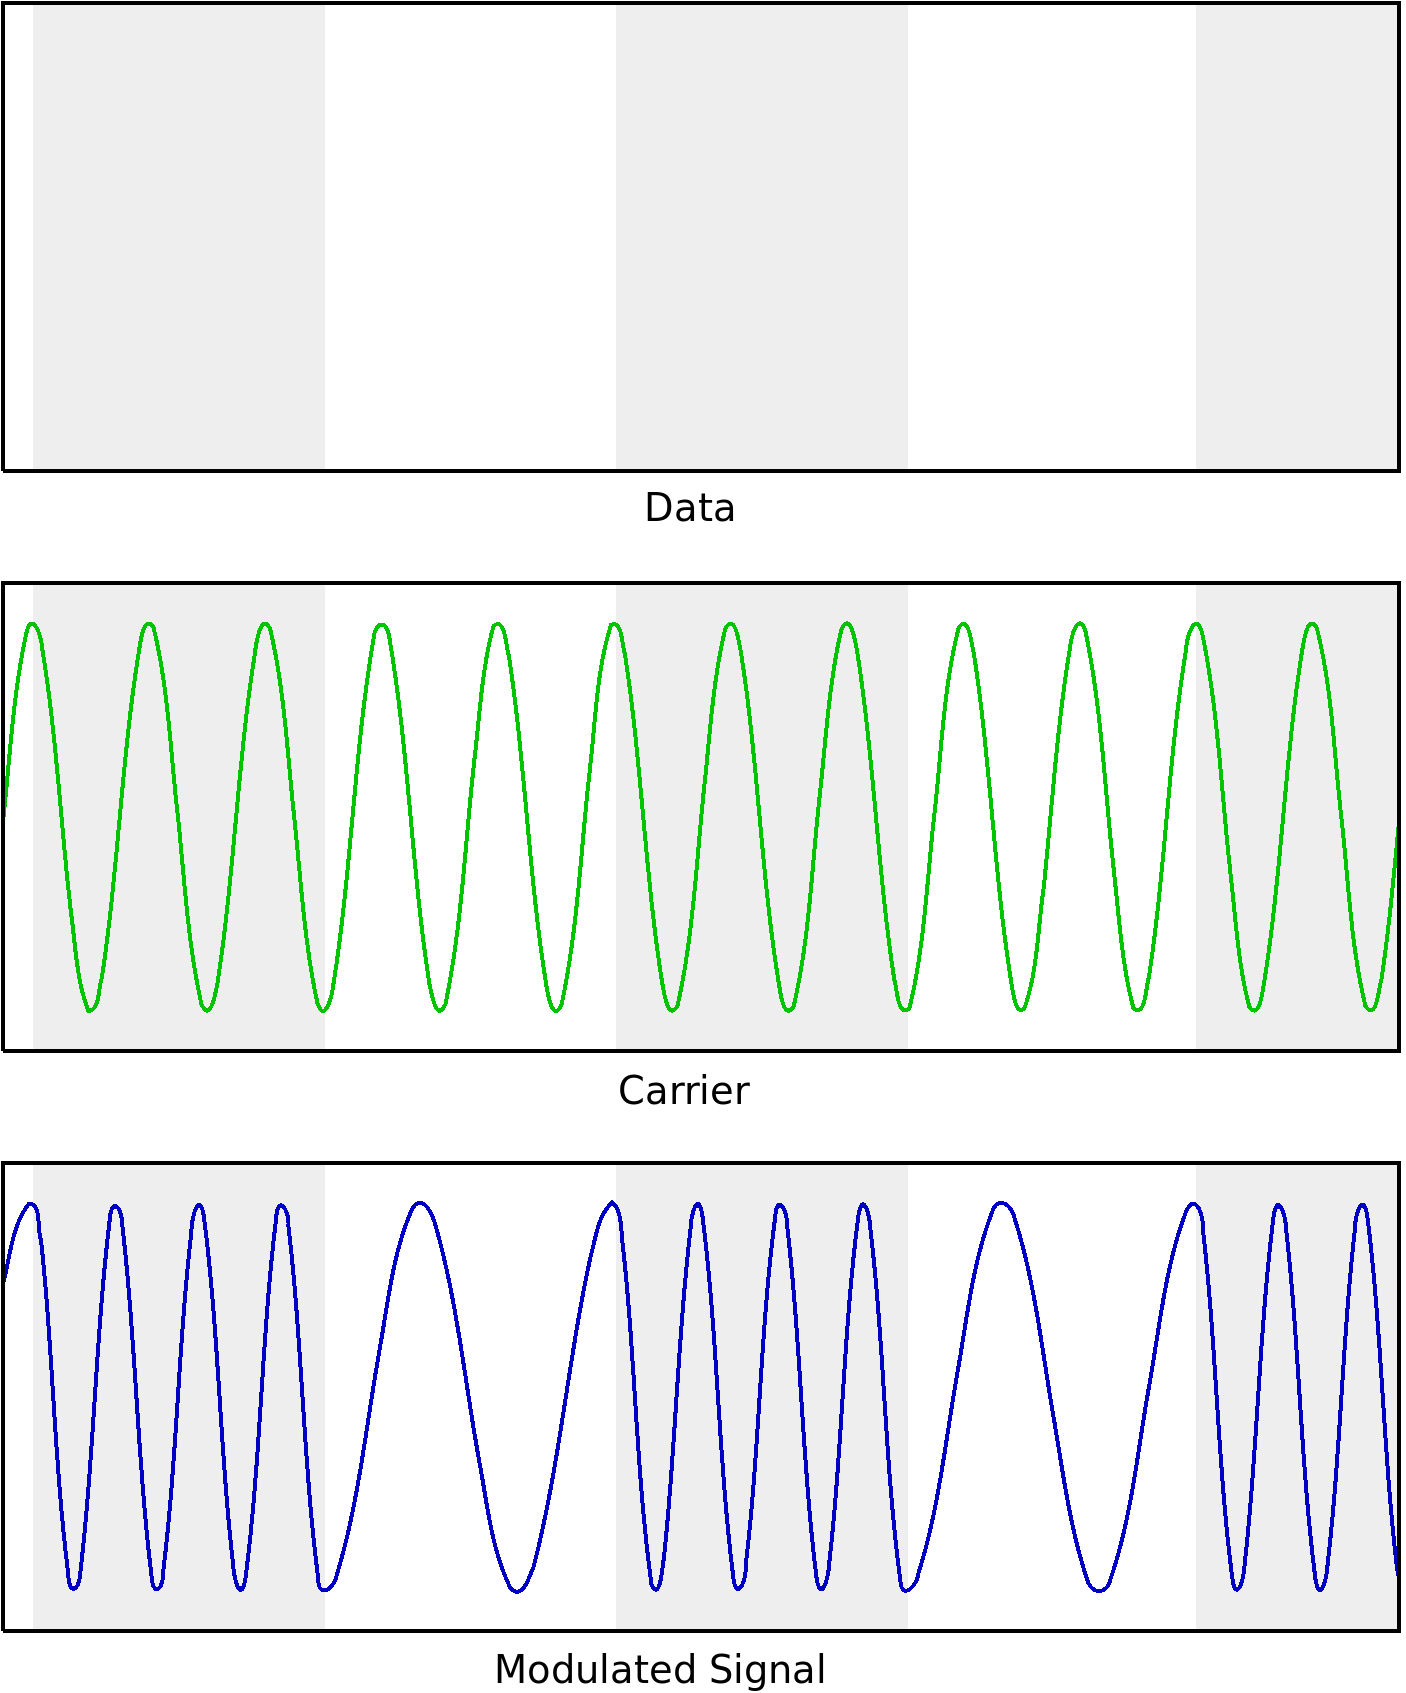
\includegraphics[width=\textwidth,height=.8\textheight,keepaspectratio]{a15/Fsk.png}\\
    {\tiny Frequenzumtastung \hyperlink{refs}{\cite{wm}}}
    \column{.55\textwidth}
    \begin{itemize}
      \item ähnlich zu FM
      \item unempfindlich gegenüber Störungen
      \item einfachste Umsetzung: mittels zweier Frequenzen übertragen
    \end{itemize}
  \end{columns}
\end{frame}

\subsection{AFSK}
\begin{frame}{Audio Frequency Shift Keying (AFSK)}
  Modulation zweier Töne, je nach Zustand
  \begin{exampleblock}{RTTY}
    \begin{description}
      \item[logisch 0] 1200\,Hz (oder 2100\,Hz bei ``high tones'')
      \item[logisch 1] 1400\,Hz (oder 2300\,Hz bei ``high tones'')
    \end{description}
    Modulation mit 14100\,kHz und SSB ergibt die Frequenzen 14101,200\,kHz und 14101,400\,kHz.\\
    Die 200\,Hz Frequenzabstand wird \emph{Shift} genannt.
  \end{exampleblock}
\end{frame}

\section{PSK}
\begin{frame}{Phase Shift Keying (PSK)}
  \begin{columns}
    \column{.5\textwidth}
    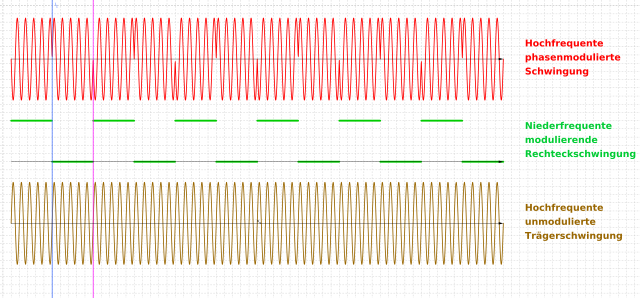
\includegraphics[width=\textwidth,height=.8\textheight,keepaspectratio]{a15/Phase_modulation_(PHM).png}\\
    {\tiny BPSK mit harter Umtastung \hyperlink{refs}{\cite{wm}}}
    \column{.45\textwidth}
    \begin{itemize}
      \item Welle wird um $180^\circ$ gedreht
      \item BPSK enthält nur zwei Zustände (binary)
    \end{itemize}
  \end{columns}
\end{frame}

\subsection{QPSK}
\begin{frame}{Quadraturphasenumtastung}
  \begin{columns}
    \column{.5\textwidth}
    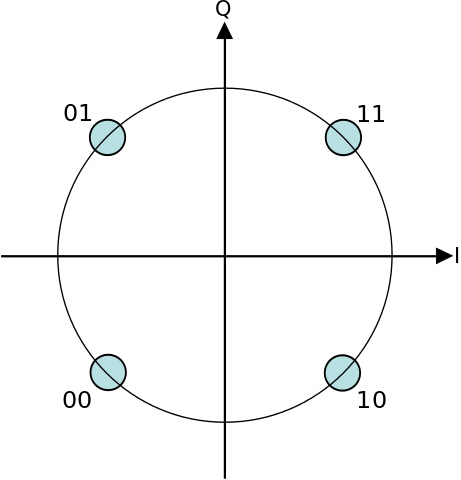
\includegraphics[width=\textwidth,height=.8\textheight,keepaspectratio]{a15/QPSK_Gray_Coded.png}\\
    {\tiny Konstellationsdiagramm QPSK (``4-QAM'')}
    \column{.45\textwidth}
    \begin{itemize}
      \item QPSK nutzt Phasensprünge alle $90^\circ$ (quadrature)
      \item $\rightarrow$ Übertragung von 2 Bits zur gleichen Zeit
      \item Verwendung bei \emph{PSK31} und \emph{Pactor}
      \item Darstellung als Konstellationsdiagramm mit \emph{I} für \emph{In-phase component} und \emph{Q} für \emph{Quadrature Component}
    \end{itemize}
  \end{columns}
\end{frame}

\subsection{QAM}
\begin{frame}{Quadraturamplitudenmodulation}
  \begin{columns}
    \column{.5\textwidth}
    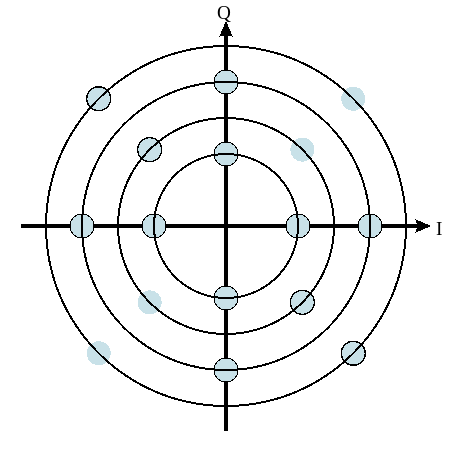
\includegraphics[width=\textwidth,height=.8\textheight,keepaspectratio]{a15/Circular_16QAM.png}\\
    {\tiny Circular 16QAM}
    \column{.45\textwidth}
    \begin{itemize}
      \item Kombination von Phase und Amplitude für Datenübertragung
      \item Mehrere Bits können zur gleichen Zeit übertragen werden
      \item Anwendung bei Modems, DSL, DVB etc.
      \item \emph{Beispiel: \href{https://upload.wikimedia.org/wikipedia/commons/9/90/QAM16_Demonstration.gif}{$\Rightarrow$ 4 Bit 16-QAM Demo}}
      \item DVB-C2 G.hn (HomeGrid) nutzen 12 Bit 4096-QAM
    \end{itemize}
  \end{columns}
\end{frame}


\section{Packet Radio}
\begin{frame}{Packet Radio}
  \begin{itemize}
    \item \ldots ist tot
    \item \ldots aber dummerweise noch Prüfungsbestandteil
    \item meist im UHF-Band, geht aber auch in VHF, KW oder SHF
    \item höhere Übertragungsraten als RTTY (i.\,d.\,R.\, 1200 oder 9600 Baud)
    \item Fehlerkorrektur
    \item Digipeater als Zwischenstationen
    \item Mailboxen für Speicherstellen
  \end{itemize}
\end{frame}

\begin{frame}{Packet Radio}
  \begin{columns}
    \column{.47\textwidth}
    1k2-Packet
    \begin{itemize}
      \item 1200\,Baud
      \item NF-Töne bei 1200\,Hz und 2200\,Hz (1000\,Hz Shift)
      \item Mittenfrequenz bei 1700\,Hz
      \item $\rightarrow$ AFSK-Signal mit 12\,kHz Bandbreite
    \end{itemize}
    \column{.47\textwidth}
    9k6-Packet
    \begin{itemize}
      \item 9600\,Baud
      \item Optimierung der Übertragung von vielen 1en oder 0en durch ``Scrambling'' (abwechselnde Invertierung)
      \item hohe Rechteckfrequenzen von 4800\,Hz werden statt über den NF-Eingang direkt in den Modulator eingespeist
      \item Bandbreite 20 kHz
    \end{itemize}
  \end{columns}
\end{frame}

\begin{frame}{TX-Delay}
  \begin{itemize}
    \item Sender braucht einige Zeit zum einschwingen
    \item Geräte brauchen Zeit, um von Empfang auf Sendung zu schalten
    \item Abhilfe schafft das einstellbare \emph{TX-Delay} am Computer, der Soundkarte oder dem TNC
    \item $\rightarrow$ mit der Datenübertragung wird einige Millisekunden gewartet
  \end{itemize}
\end{frame}

\begin{frame}{Packet Radio Netzwerk}
  \begin{itemize}
    \item es kann immer nur eine Station gleichzeitig senden\footnote{wie im 10BASE2-Netzwerk oder mit Hubs}
    \item ansonsten kommt es zu Kollisionen
    \item $\rightarrow$ \emph{DAMA} (Demand Assigned Multiple Access)
    \item Stationen werden nacheinander gepollt, ob sie Daten senden möchten\footnote{fast wie bei Token Ring}
  \end{itemize}
\end{frame}

\subsection{APRS}
\begin{frame}{Automatic Packet Reporting System (APRS)}
  \begin{itemize}
    \item sendet kurze Datenpakete ohne Bestätigung
    \item Inhalte sind Wetterdaten, Positionsmeldungen und andere Messwerte
    \item ganz häufig GPS-Koordinaten des eigenen Fahrzeugs mit Rufzeichen
    \item Darstellung mit Karte unter \url{http://aprs.fi/\#!addr=berlin}
    \item QRG ist 144,800\,MHz
  \end{itemize}
\end{frame}

\section{PSK31}
\begin{frame}{PSK31}
  \begin{itemize}
    \item 1999 von G3LPX entwickelt
    \item Bitrate von 31,25\,Bit/s -- Bandbreite somit 31\,Hz
    \item $\rightarrow$ 1/10 der Bandbreite von Telegraphie!
    \item mit guten Filtern reichen 10\,W für weltweiten Funkverkehr
    \item Subarten BPSK und QPSK (mit Fehlerkorrektur auf zweitem Kanal)
    \item Hilfsträger bei 1000\,Hz
  \end{itemize}
\end{frame}

\section{AMTOR}
\begin{frame}{AMTOR}
  Amateur Microprocessor Teleprinting Over Radio
  \begin{itemize}
    \item hohe Übertragungssicherheit
    \item nach drei Zeichen wird eine Quittierung eingefordert
    \item $\rightarrow$ ARQ (automatic repeat request)
    \item 7 Bits, von denen nur die 38 Kombinationen mit 4 Einsen und 3 Nullen verwendet werden
    \item abgelöst durch PACTOR
  \end{itemize}
\end{frame}

\section{PACTOR}
\begin{frame}{PACTOR}
  Packet Teleprinting Over Radio
  \begin{itemize}
    \item Weiterentwicklung von AMTOR durch DF4KV und DL6MAA in 1990
    \item für störungsbehaftete Übertragung auf Kurzwelle geeignet
    \item 8-Bit Code zzgl. CRC-Check
    \item Weiterentwicklung aktuell bei PACTOR 4 mit 10500\,bps
    \item Controller ist gebrauchsmustergeschützt und recht teuer
  \end{itemize}
\end{frame}


\renewcommand{\refname}{Referenzen}

\hypertarget{refs}{}
\textcolor{white}{} \\ %\vspace{} geht nicht
\Large Referenzen/Links
\footnotesize

\begin{thebibliography}{}
  \bibitem{darc}  DARC Online-Lehrgang Lektion A15:\\
    \url{https://www.darc.de/der-club/referate/ajw/lehrgang-ta/a15/}
  \bibitem{wm} 	Wikimedia:\\
    \href{https://de.wikipedia.org/wiki/Digitalsignal#/media/File:\%C3\%9Cbersicht_kontinuierliche_und_diskrete_Signale.svg}{\mbox{Übersicht kontinuierliche und diskrete Signale, By wdwd (Own work) [GFDL (http://www.gnu.org/copyleft/fdl.html) or CC BY 3.0 (http://creativecommons.org/licenses/by/3.0)], via Wikimedia Commons}}\\
    \href{https://commons.wikimedia.org/wiki/Category:Quantized_QAM?uselang=de#/media/File:Circular_16QAM.svg}{\mbox{von Life of Riley (Eigenes Werk) [Public domain], via Wikimedia Commons}}\\
    \href{https://de.wikipedia.org/wiki/Phasenmodulation#/media/File:Phase_modulation_(PHM).svg}{\mbox{By L31n42 (Own work) [CC0], via Wikimedia Commons}}\\
    \href{https://de.wikipedia.org/wiki/Quadraturphasenumtastung#/media/File:QPSK_Gray_Coded.svg}{\mbox{By No machine-readable author provided. Splash assumed (based on copyright claims). [GFDL (http://www.gnu.org/copyleft/fdl.html), CC-BY-SA-3.0 (http://creativecommons.org/licenses/by-sa/3.0/) or CC BY-SA 2.5-2.0-1.0 (http://creativecommons.org/licenses/by-sa/2.5-2.0-1.0)], via Wikimedia Commons}}\\
    \href{https://de.wikipedia.org/wiki/Frequenzumtastung#/media/File:Fsk.svg}{\mbox{Bildung eines binären FSK Signals, By No machine-readable author provided. Ktims assumed (based on copyright claims). [GFDL (http://www.gnu.org/copyleft/fdl.html), CC-BY-SA-3.0 (http://creativecommons.org/licenses/by-sa/3.0/) or CC BY-SA 2.5-2.0-1.0 (http://creativecommons.org/licenses/by-sa/2.5-2.0-1.0)], via Wikimedia Commons}}

  \bibitem{wp}    Wikipedia - Die freie Enzyklopädie:\\
  \bibitem{bna}   Fragenkatalog Bundesnetzagentur Technik Klasse A:\\
    \url{https://www.bundesnetzagentur.de/SharedDocs/Downloads/DE/Sachgebiete/Telekommunikation/Unternehmen_Institutionen/Frequenzen/Amateurfunk/Fragenkatalog/TechnikFragenkatalogKlasseAf252rId9014pdf.pdf?__blob=publicationFile&v=3}
\end{thebibliography}

% Hier könnte noch eine Kontaktfolie stehen

\end{document}

